\documentclass[tikz]{standalone}

\usepackage{amsmath}
\usepackage{physics}

\usetikzlibrary{arrows.meta,positioning}

\begin{document}
	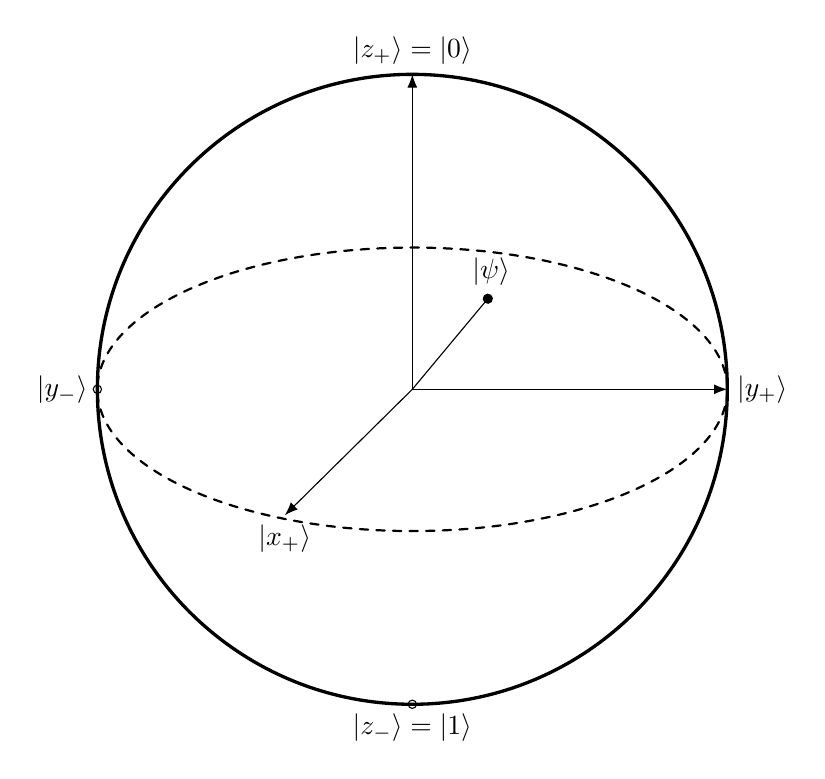
\begin{tikzpicture}[line cap=round, line join=round]
		\draw[very thick] (0,0) circle (4cm);
		\draw[thick, rotate around={0.:(0.,0.)}, dash pattern=on 3pt off 3pt] (0,0) ellipse (4cm and 1.8cm);
		\draw[-Circle] (0,0) -- (1,1.2) node[above]{$\ket{\psi}$};

		\draw[-Latex] (0,0) -- (0,4) node[above]{$\ket{z_+}=\ket{0}$};
		\draw[-Latex] (0,0) -- (-1.62,-1.6) node[below]{$\ket{x_+}$};
		\draw[-Latex] (0,0) -- (4,0) node[right]{$\ket{y_+}$};

%		\draw[fill] (0,0) circle (1.5pt);
		
		\draw (0,-4) circle (1.5pt) node[below] {$\ket{z_-}=\ket{1}$};
		\draw (-4,0) circle (1.5pt) node[left] {$\ket{y_-}$};
	\end{tikzpicture}
\end{document}